\section{Antenna Design 1 -- Monopole}
\fixme{Update captions or labels. Copy from next section, maybe.}

\subsection{Read Mode}
\begin{figure}[htbp]
   \begin{subfigure}[b]{0.49\linewidth}
        \centering
        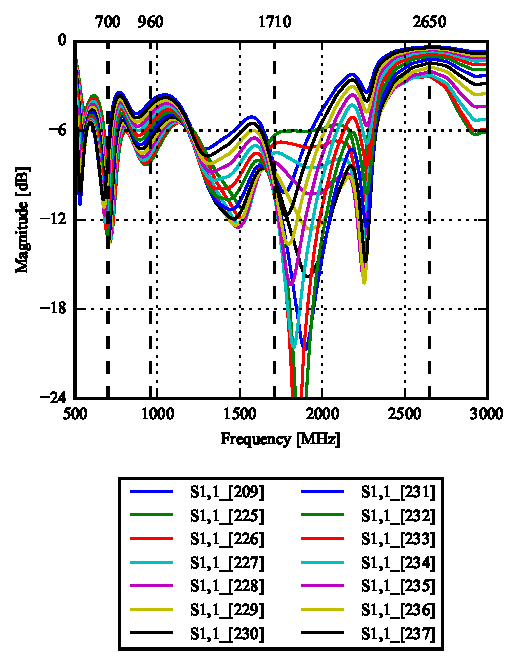
\includegraphics{img/tech_sol/monopole/read_mode/s11}
        \caption{$S_{11}$, sweeping $C_1$ and fixing $C_2$.}
        \label{fig:ant1_s11}
    \end{subfigure}
    \hfill
    \begin{subfigure}[b]{0.49\linewidth}
        \centering
        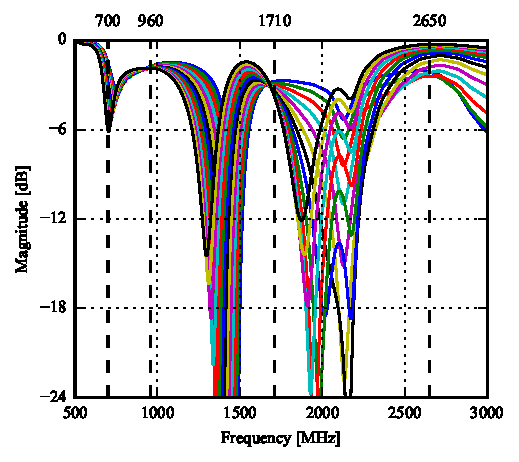
\includegraphics{img/tech_sol/monopole/read_mode/s22}
        \caption{$S_{11}$, sweeping $C_1$ and fixing $C_2$.}
        \label{fig:ant1_s22}
    \end{subfigure}
~
    \begin{subfigure}[b]{0.49\linewidth}
        \centering
        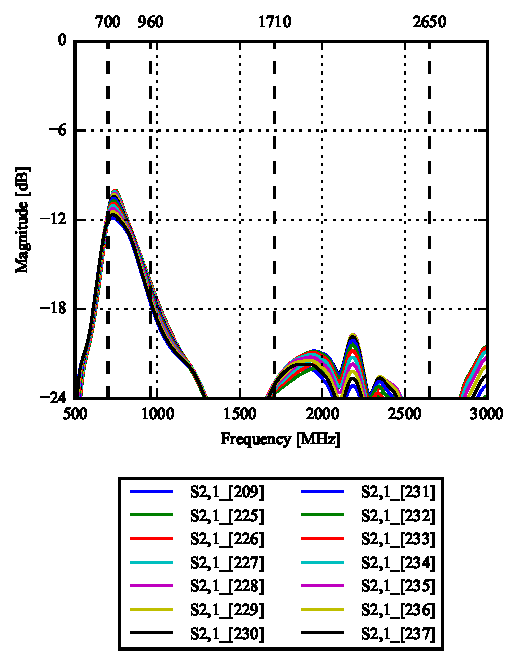
\includegraphics{img/tech_sol/monopole/read_mode/s21_s11}
        \caption{$S_{21}$ with $C_2$ = \SI{0.3}{pF} and $C_1$ varying from \SI{0.3}{pF} to \SI{2.9}{pF}.}
        \label{fig:ant1_s11}
    \end{subfigure}
    \hfill
    \begin{subfigure}[b]{0.49\linewidth}
        \centering
        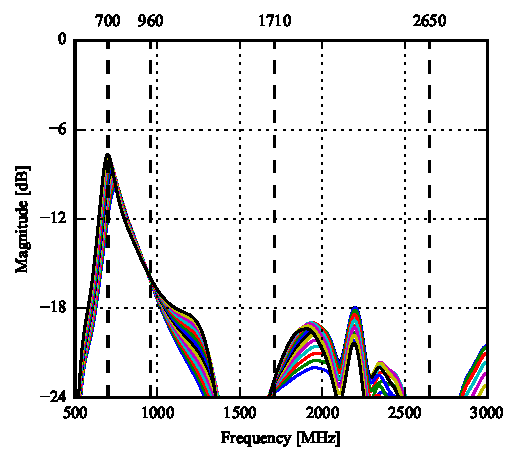
\includegraphics{img/tech_sol/monopole/read_mode/s21_s22}
        \caption{$S_{21}$ with $C_2$ = \SI{0.3}{pF} and $C_1$ varying from \SI{0.3}{pF} to \SI{2.9}{pF}.}
        \label{fig:ant1_s22}
    \end{subfigure}
    \caption{Parameter sweep for tuning the shunt capacitor of each antenna, $C_1$ and $C_2$ for port 1 and 2, respectively. Port 1 is the top antenna and port 2 is the side antenna.}
    \label{fig:sparam_mono}
\end{figure}


\subsection{Play Mode}
\begin{figure}[htbp]
   \begin{subfigure}[b]{0.49\linewidth}
        \centering
        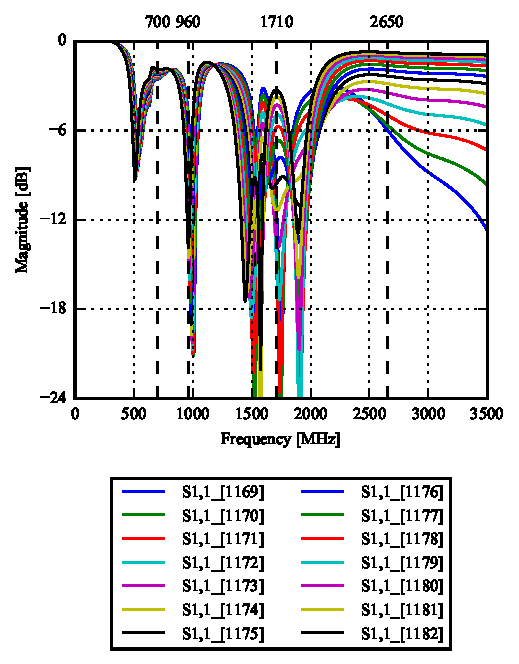
\includegraphics{img/tech_sol/monopole/play_mode/s11}
        \caption{$S_{11}$, sweeping $C_1$ and fixing $C_2$.}
        \label{fig:ant1_s11}
    \end{subfigure}
    \hfill
    \begin{subfigure}[b]{0.49\linewidth}
        \centering
        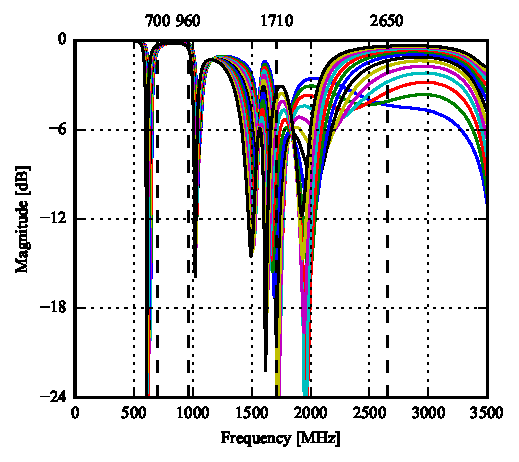
\includegraphics{img/tech_sol/monopole/play_mode/s22}
        \caption{$S_{11}$, sweeping $C_1$ and fixing $C_2$.}
        \label{fig:ant1_s22}
    \end{subfigure}
~
    \begin{subfigure}[b]{0.49\linewidth}
        \centering
        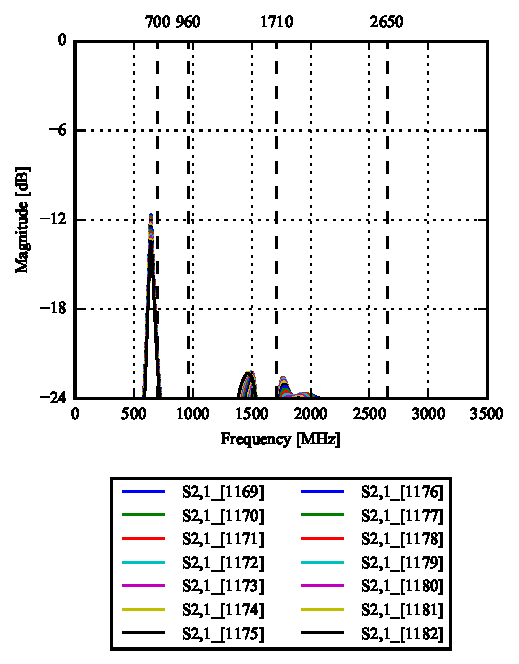
\includegraphics{img/tech_sol/monopole/play_mode/s21_s11}
        \caption{$S_{21}$ with $C_2$ = \SI{0.3}{pF} and $C_1$ varying from \SI{0.3}{pF} to \SI{2.9}{pF}.}
        \label{fig:ant1_s11}
    \end{subfigure}
    \hfill
    \begin{subfigure}[b]{0.49\linewidth}
        \centering
        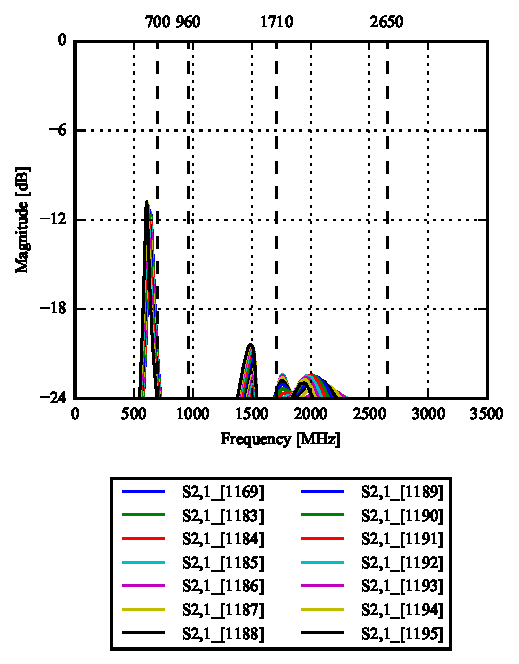
\includegraphics{img/tech_sol/monopole/play_mode/s21_s22}
        \caption{$S_{21}$ with $C_2$ = \SI{0.3}{pF} and $C_1$ varying from \SI{0.3}{pF} to \SI{2.9}{pF}.}
        \label{fig:ant1_s22}
    \end{subfigure}
    \caption{Parameter sweep for tuning the shunt capacitor of each antenna, $C_1$ and $C_2$ for port 1 and 2, respectively. Port 1 is the top antenna and port 2 is the side antenna.}
    \label{fig:sparam_mono}
\end{figure}

\subsection{Talk Mode}
\begin{figure}[htbp]
   \begin{subfigure}[b]{0.49\linewidth}
        \centering
        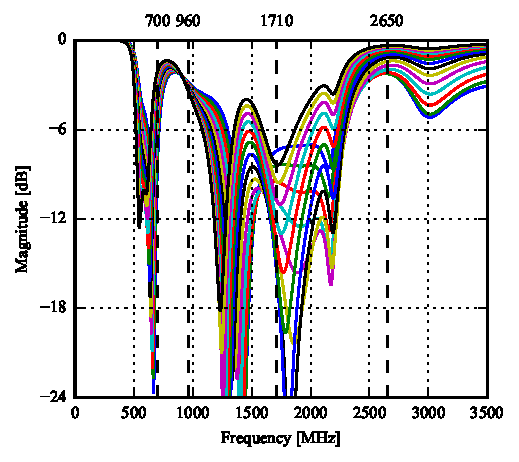
\includegraphics{img/tech_sol/monopole/talk_mode/s11}
        \caption{$S_{11}$, sweeping $C_1$ and fixing $C_2$.}
        \label{fig:ant1_s11}
    \end{subfigure}
    \hfill
    \begin{subfigure}[b]{0.49\linewidth}
        \centering
        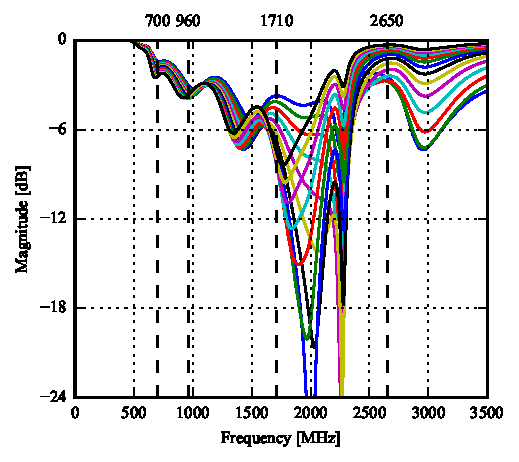
\includegraphics{img/tech_sol/monopole/talk_mode/s22}
        \caption{$S_{11}$, sweeping $C_1$ and fixing $C_2$.}
        \label{fig:ant1_s22}
    \end{subfigure}
~
    \begin{subfigure}[b]{0.49\linewidth}
        \centering
        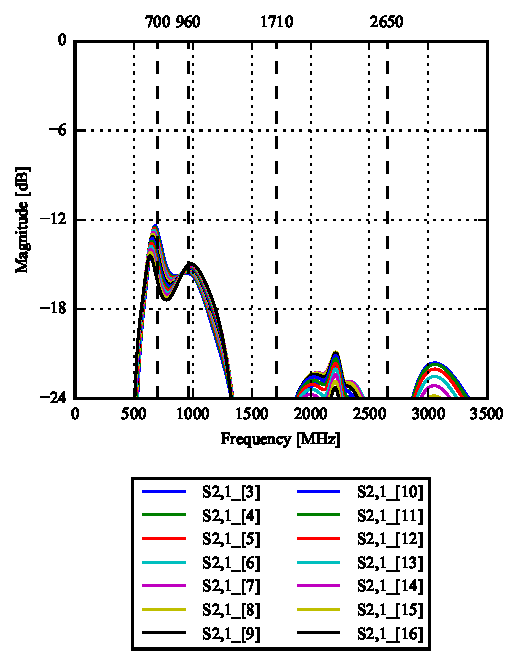
\includegraphics{img/tech_sol/monopole/talk_mode/s21_s11}
        \caption{$S_{21}$ with $C_2$ = \SI{0.3}{pF} and $C_1$ varying from \SI{0.3}{pF} to \SI{2.9}{pF}.}
        \label{fig:ant1_s11}
    \end{subfigure}
    \hfill
    \begin{subfigure}[b]{0.49\linewidth}
        \centering
        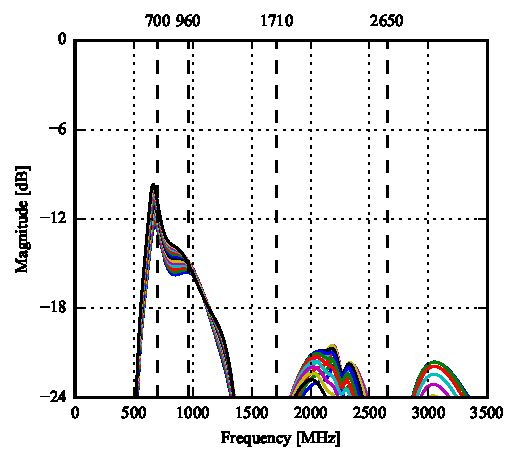
\includegraphics{img/tech_sol/monopole/talk_mode/s21_s22}
        \caption{$S_{21}$ with $C_2$ = \SI{0.3}{pF} and $C_1$ varying from \SI{0.3}{pF} to \SI{2.9}{pF}.}
        \label{fig:ant1_s22}
    \end{subfigure}
    \caption{Parameter sweep for tuning the shunt capacitor of each antenna, $C_1$ and $C_2$ for port 1 and 2, respectively. Port 1 is the top antenna and port 2 is the side antenna.}
    \label{fig:sparam_mono}
\end{figure}

\subsection{SAR}

